% !TEX encoding = UTF-8
% !TEX TS-program = pdflatex
% !TEX root = ../tesi.tex
% !TEX spellcheck = it-IT

%**************************************************************
\chapter{Descrizione dello stage}
\label{cap:descrizione-stage}
%**************************************************************

%\intro{Breve introduzione al capitolo}\\

%**************************************************************
%\section{Analisi preventiva dei rischi}

%Durante la fase di analisi iniziale sono stati individuati alcuni possibili rischi a cui si potrà andare incontro.
%Si è quindi proceduto a elaborare delle possibili soluzioni per far fronte a tali rischi.\\

%\begin{risk}{Performance del simulatore hardware}
%    \riskdescription{le performance del simulatore hardware e la comunicazione con questo potrebbero risultare lenti o non abbastanza buoni da causare il fallimento dei test}
%    \risksolution{coinvolgimento del responsabile a capo del progetto relativo il simulatore hardware}
%    \label{risk:hardware-simulator} 
%\end{risk}

%**************************************************************
\section{Obiettivi dello stage}
\label{obiettivi}
Sulla base della durata dello stage, l'azienda ha fissato degli obiettivi che si aspettava di veder raggiunti entro il termine del rapporto lavorativo. In particolare veniva richiesta:
\begin{itemize}
\item Conoscenza degli applicativi di Mediana S.r.l.u., in particolare di CSIndex nella sua ultima versione NPS EBS;
\item Conoscenza delle fasi consulenziali come:
	\begin{itemize}
	\item Redazione di \textit{test book} per U.A.T.\footnotemark[1];
	\item Test e verifiche dei programmi presi in esame;
	\item Redazione di manuali propedeutici al \textit{roll out} dell'applicativo.
	\end{itemize}
\item Apprendimento del \gls{data model} di NPS EBS;
\item Sviluppare una buona autonomia nella progettazione e sviluppo di \textit{statement} SQL.
\end{itemize}

\section{Calendario delle attività}
\label{calendario}
Nel dettaglio il lavoro è stato suddiviso nel seguente modo:
\begin{enumerate}
\item \textbf{Settimana 1}: introduzione ai prodotti aziendali e alla metodologie di lavoro in Mediana S.r.l.u.;
\item \textbf{Settimana 2}: focalizzazione sul prodotto NPS EBS e condivisione della documentazione inerente a questo progetto;
\item \textbf{Settimana 3}: esecuzione dei test funzionali descritti negli U.A.T in affiancamento al tutor;
\footnotetext[1]{Test visti in un punto della \hyperref[fasi progetto]{Sezione 1.4.2}}
\item \textbf{Settimana 4}: aggiornamento dei manuali per le diverse categorie di utente previste all'interno dell'applicativo;
\item \textbf{Settimana 5-6}: conoscenza del codice dell'applicativo e della struttura del \textit{database} in affiancamento agli sviluppatori;
\item \textbf{Settimana 7-8}: \textit{support} di NPS EBS fino al rilascio in PROD\footnotemark[2] 
\footnotetext[2]{Uno degli ambienti trattati nella \hyperref[ambienti programma]{Sezione 1.4.3}};
\end{enumerate}

Per una più chiara panoramica di questa suddivisione, nella \hyperref[gantt attivita]{Figura 3.1} riporto il \gls{diagramma di Gantt} con il calendario di tutte le attività svolte durante il periodo di stage.

\begin{figure}[h!]
\begin{center}
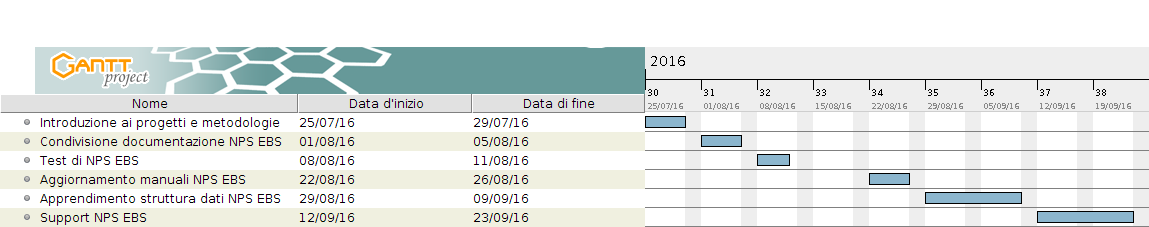
\includegraphics[scale=0.32]{Gantt} 
\caption{Diagramma di Gantt delle attività svolte}
\label{gantt attivita}
\end{center}
\end{figure}
\FloatBarrier

\section{Suddivisione dello stage e motivo della scelta}
Dal calendario si evince che lo stage è stato caratterizzato da due periodi distinti che sono identificabili nel modo seguente:
\begin{itemize}
\item Le prime quattro settimane sono servite inizialmente per apprendere il lavoro di consulente tecnico per poi metterlo in pratica con test e stesura dei manuali utente;
\item Le ultime quattro settimane invece sono state contraddistinte da un lavoro che si addice più che altro a uno sviluppatore, infatti tramite alcune operazioni di \textit{bug-fixing} ho potuto metter mano sia al codice, apprendendo così parte della logica che costituisce il programma NPS, sia al \textit{database}, capendo come vengono strutturati e suddivisi i dati che costituiscono il sistema.
\end{itemize}
Questa particolare suddivisione è dovuta al fatto che Mediana S.r.l.u. cercava un pretendente per lo stage che riuscisse a impersonificare una figura professionale di consulente che però all'occorrenza sapesse anche mettere le mani al codice degli applicativi presi in esame.
Con queste prerogative l'azienda aveva infatti deciso di partecipare a Stage IT 2016 (logo nella \hyperref[stage IT]{Figura 3.2}), un evento organizzato da Confindustria Padova in collaborazione con le Università di Padova e Venezia per favorire gli incontri tra aziende e studenti nell'ottica di un futuro possibile stage.

\begin{figure}[h!]
\begin{center}

\includegraphics[scale=0.27]{stageIT}
\caption{Logo di Stage IT 2016}
\label{stage IT}
\end{center}
\end{figure}
\FloatBarrier

Nonostante non fosse stato definito un progetto in particolare, ma venisse data semplicemente l'opportunità all'aspirante tirocinante di essere inserito all'interno di un progetto che fosse in corso durante il periodo nel quale egli si sarebbe presentato; ho deciso, dopo un secondo colloquio, di sostenere questo stage presso Mediana S.r.l.u. sia poiché ho valutato questo genere di lavoro potenzialmente interessante sia perché a prima vista il team mi è sembrato molto unito e allo stesso tempo competente.

\section{Prima fase di stage}
\label{prima fase}
In dettaglio, durante la prima metà del mio stage, il mio tutor aziendale, che per il progetto NPS svolge sia il ruolo di consulente che di project manager, mi ha prima esposto quelli che sono gli incarichi di un consulente tecnico in Mediana S.r.l.u., facendomeli poi provare di persona inizialmente affiancandomi per poi lasciarmi sempre più in autonomia. Detto ciò, approfondendo quanto già accennato nella \hyperref[organizzazione]{Sezione 1.2}, adesso vado a descrivere quali sono le attività che caratterizzano questo ruolo, basandomi sull'esperienza vissuta durante lo stage.

\subsection{Studio della documentazione}
Innanzitutto ci tengo a precisare che ci sono state diverse occupazioni delle quali purtroppo non sono stato incaricato, vista sia la fase nel quale il progetto era giunto, sia l'importanza fondamentale di alcune attività che non potevano di certo essere lasciate fare a uno stagista che non avesse mai avuto un esperienza del genere sul campo. Partendo proprio da quest'ultime le più importanti sono sicuramente le interazioni con il cliente, che esse siano tramite \textit{call} o \textit{e-mail}, alle quali ho per lo meno potuto assistere. Così facendo mi sono reso conto che in aggiunta alle motivazioni enunciate, prima di poter essere utile a questa causa, avrei avuto bisogno di molto più tempo per comprendere nella sua interezza il \textit{software} NPS. \\ Per colmare quest'ultima lacuna la prima cosa che ho fatto è stata leggere la versione originale del B.O.R\footnotemark[3] definito al tempo dal committente EBS, del quale è possibile vedere un esempio di pagina nella \hyperref[bor]{Figura 3.3}.
 
\begin{figure}[h!]
\begin{center}
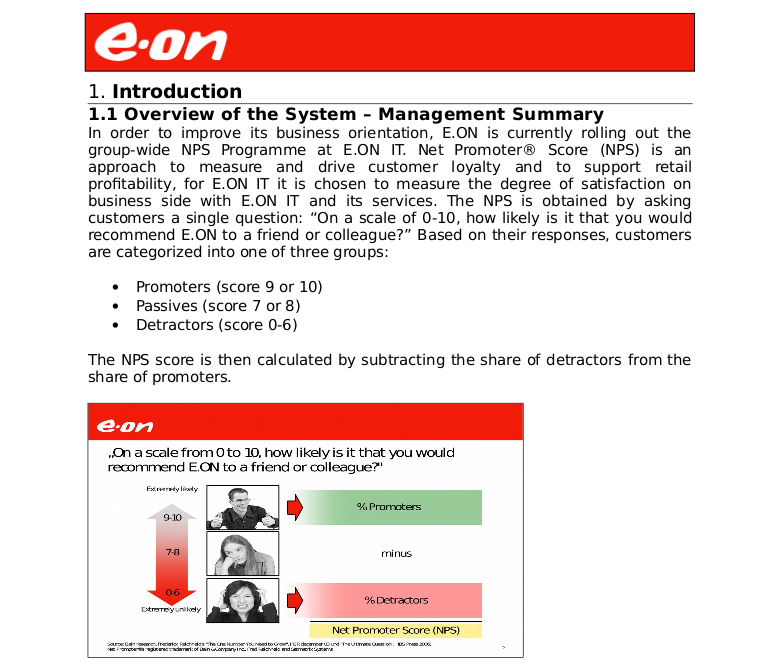
\includegraphics[scale=0.5]{BOR}
\caption{Primo caitolo del B.O.R. di NPS EBS}
\label{bor}
\end{center}
\end{figure}
\FloatBarrier

Questo documento mi ha permesso di avere una visione d'insieme su NPS, che ho descritto nel dettaglio nel \hyperref[cap:progetto-stage]{Capitolo 2}, e su quello che il cliente al tempo aveva richiesto. In questo modo ho potuto notare alcune differenze che ci sono rispetto all'ultima versione, e che poi ho ritrovato evidenziate nel secondo documento che ho visionato, ovvero il B.B.P.\footnotemark[3]
\footnotetext[3]{Per chiarimenti sulla documentazione vedere la \hyperref[fasi progetto]{Sezione 1.4.2}} 
del così detto \textit{sprint} 3, le cui pagine, strutturate come nella \hyperref[bbp]{Figura 3.4}, contengono per l'appunto le ultime \acrshort{cr} e le nuove funzionalità che sono state richieste dal committente e che sono state implementate prima del mio arrivo in azienda.

\begin{figure}[h!]
\begin{center}
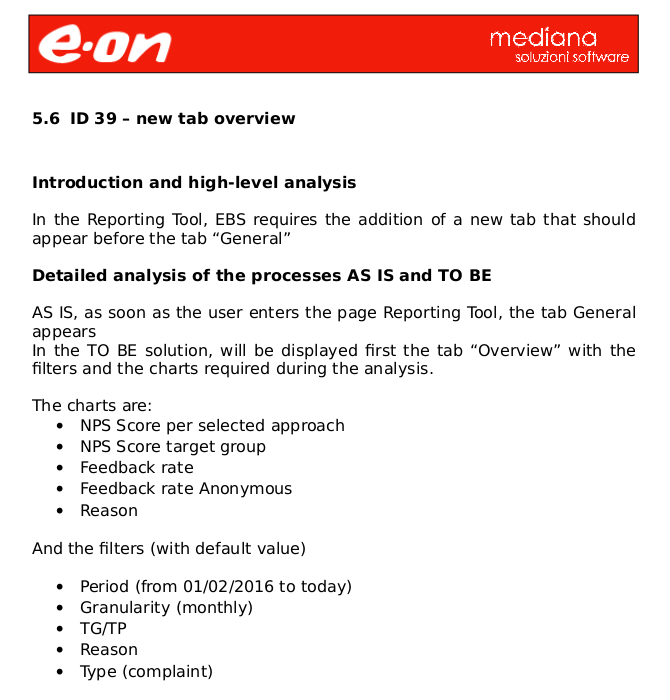
\includegraphics[scale=0.5]{BBP}
\caption{Esempio di soluzione proposta nel B.B.P. sprint 3 di NPS EBS}
\label{bbp}
\end{center}
\end{figure}
\FloatBarrier

Essendo arrivati ormai nel periodo conclusivo di questo \textit{sprint}, come dicevo precedentemente, non ho potuto assistere di persona a diversi passaggi di natura consulenziale, come tutta la fase di analisi e di pianificazione fino alla stesura stessa del B.B.P., ma per lo meno recuperando questa documentazione sono riuscito a capire meglio la situazione in cui il progetto si trovava. %\\

\subsection{Test e tracciamento dei bug}
\label{test}
A questo punto il mio tutor ha definito gli U.A.T. all'interno di un \textit{file} Excel condiviso su \textit{Google Drive} che io ho utilizzato sia per comprendere meglio tutte le modifiche che erano state proposte nel B.B.P. sia che per il loro scopo principale, ovvero verificare che le funzionalità dell'applicativo che sono state modificate, funzionassero effettivamente nel modo corretto. \\
Nelle figure \hyperref[indice UAT]{3.5} e \hyperref[test case]{3.6} si possono vedere alcuni esempi di come sono strutturate le pagine di questo \textit{test book}.

\begin{figure}[h!]
\begin{center}
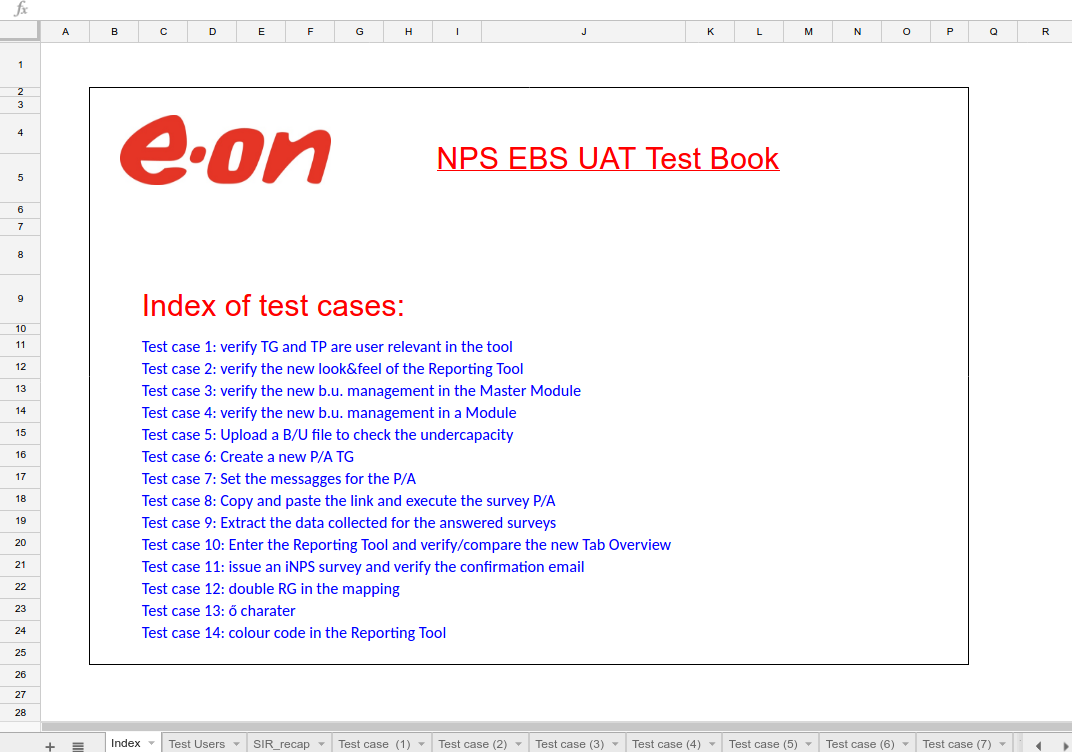
\includegraphics[scale=0.34]{indiceUAT}
\caption{Indice degli U.A.T per NPS EBS}
\label{indice UAT}
\end{center}
\end{figure}
\FloatBarrier

\begin{figure}[h!]
\begin{center}
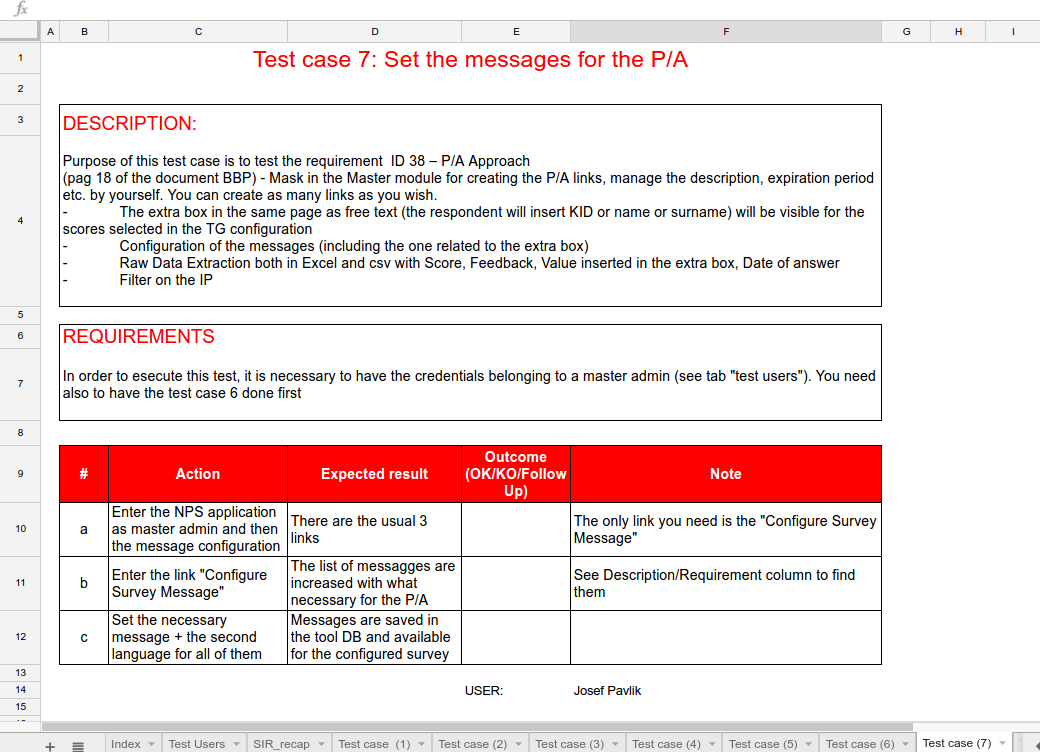
\includegraphics[scale=0.34]{testcaseUAT}
\caption{Esempio di U.A.T per NPS EBS}
\label{test case}
\end{center}
\end{figure}
\FloatBarrier

Successivamente anche il responsabile dell'azienda committente ha utilizzato il medesimo \textit{file} per testare il \textit{software} e per questo motivo a lui è stato riservato un particolare foglio chiamato SIR recap, nel quale ha potuto segnalare i \textit{bug} riscontrati assegnando ad essi diverse priorità (nella \hyperref[sir]{Figura 3.7} si può vedere una parte della lista da lui stilata).

\begin{figure}[h!]
\begin{center}
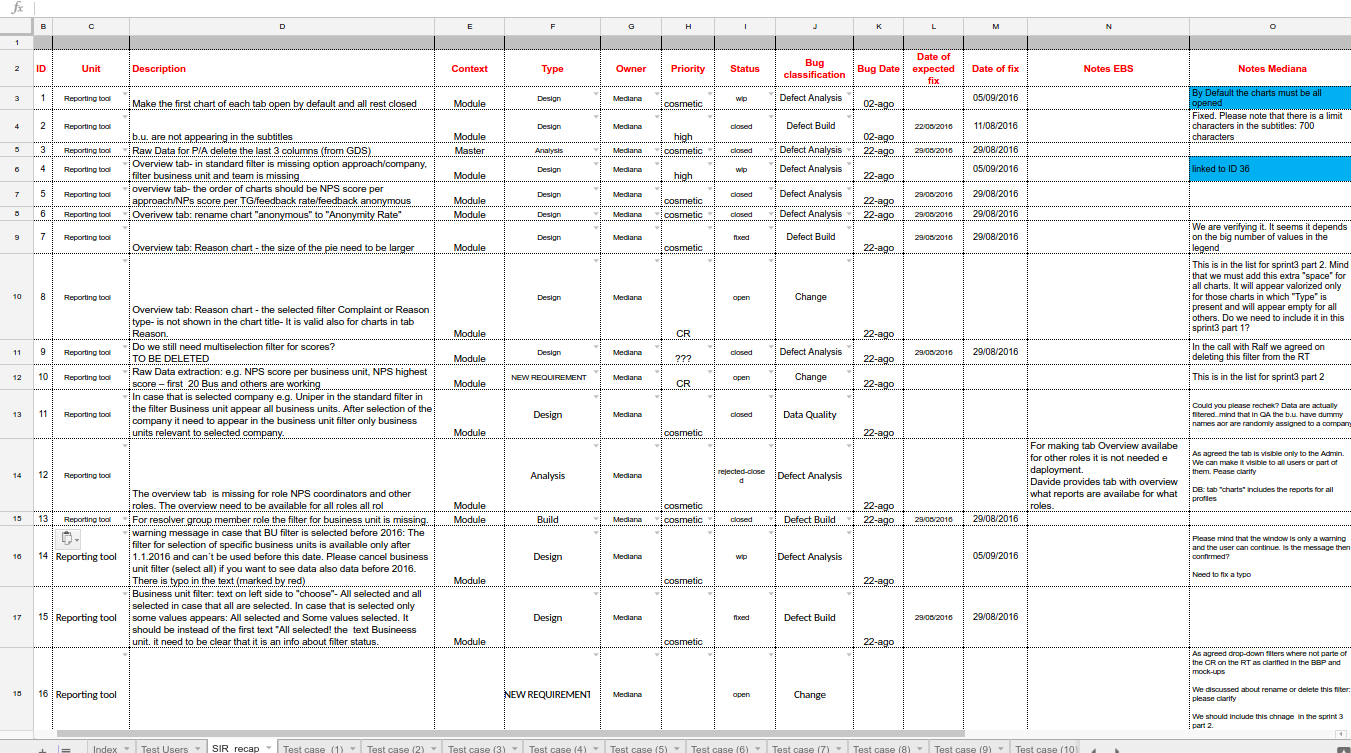
\includegraphics[scale=0.26]{SIR}
\caption{SIR recap compilato dal committente}
\label{sir}
\end{center}
\end{figure}
\FloatBarrier

Ognuna qualvolta veniva riscontrato un \textit{bug}, sia che esso venisse segnalato dal committente nel SIR recap sia che venisse individuato da me o il mio tutor, noi consulenti avevamo il compito di aggiungerlo come \textit{task} su un foglio di calcolo, riservato ai soli membri del \textit{team} che hanno seguito questo progetto. Questi \textit{bug} venivano assegnati agli sviluppatori che avevano il compito di cambiare lo stato dei \textit{task} segnalati come \textit{OPEN}, in \textit{WIP} (\emph{Work In Progess}) o \textit{CLOSED} a seconda del caso in cui essi ci avessero iniziato a lavorare o se lo avessero completato. Le altre colonne presenti in questa tabella identificano le date nelle quali venivano riscontrati i \textit{bug}, quelle di presunto rilascio e quelle di effettivo completamento. Ad ogni \textit{bug} veniva infine associata una descrizione, la pagina dell'applicativo corrispondente e una priorità a seconda di quanto fosse grave. \\ Utilizzandolo in questo modo, il \textit{file} Excel, del quale è possibile vedere una parte nella \hyperref[bug-report]{Figura 3.8}, andava ad assumere a tutti gli effetti lo stesso valore di un qualsiasi \gls{sistema di ticketing}.

\newpage
\begin{figure}[h!]
\begin{center}
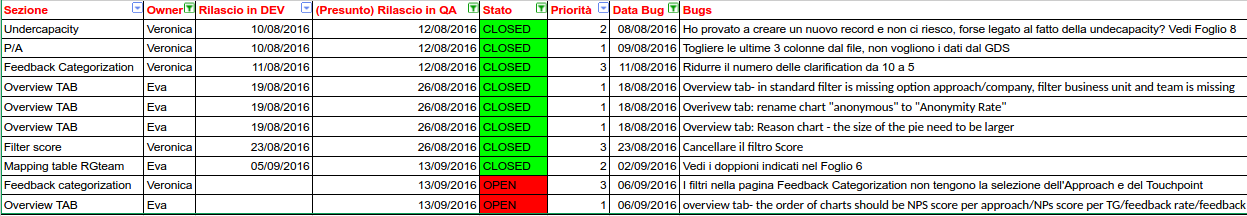
\includegraphics[scale=0.29]{Ticketing}
\caption{Foglio di calcolo utilizzato come sistema di ticketing}
\label{bug-report}
\end{center}
\end{figure}
\FloatBarrier

Fino ad avvenuto rilascio in PROD dell'applicativo, non è bastata un unica verifica delle funzionalità ma anzi, ad ogni nuovo rilascio in QA delle correzioni effettuate, ho ripetuto tutti gli U.A.T. dall'inizio in modo da verificare che a tutti gli effetti le modifiche fossero consistenti e che quindi i \textit{bug} fossero stati definitivamente risolti. Ciò è servito inoltre a verificare che non si fossero generate nuove situazione erronee dovute ai cambiamenti effettuati al codice o al passaggio di ambiente, nel quale qualcosa poteva non essere andata nel verso giusto.

\subsection{Manualistica}
\label{manuali}
Nell'ultima parte di questa prima fase di stage sono infine stato incaricato di un compito molto importante, ovvero correggere e ampliare, con le modifiche effettuate e le nuove funzionalità, tutti i manuali per ognuno dei ruoli esistenti all'interno di NPS. Questi ultimi differiscono fra loro in base agli incarichi che gli utenti hanno all'interno del sistema, dovuti al fatto che esistono diverse responsabilità o aree di pertinenza (geografiche o professionale) in EBS. \\
Durante la ristesura dei manuali, oltre a descrivere testualmente i vari passaggi che andavano svolti, ho aggiunto per ogni nuova funzione degli \gls{screenshot}, che consentono all'utente di individuare più chiaramente dove vanno applicate queste particolari azioni, come è stato fatto per esempio nella sezione che viene riportata nella \hyperref[manuale]{Figura 3.9}.

\begin{figure}[h!]
\begin{center}
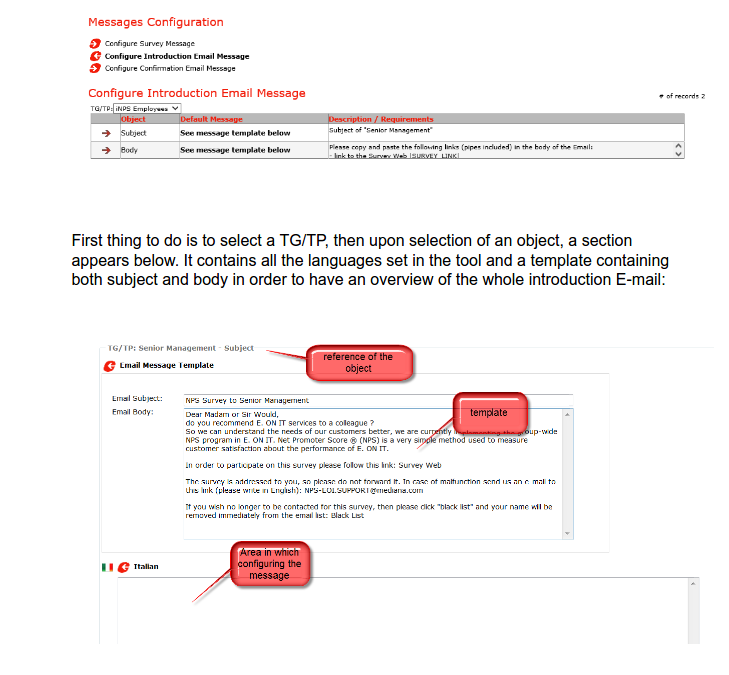
\includegraphics[scale=0.5]{manuale}
\caption{Pagina di un manuale contenente uno screenshot chiarificante}
\label{manuale}
\end{center}
\end{figure}
\FloatBarrier
 
\newpage
\section{Seconda fase di stage}
\label{seconda fase}
Per quanto riguarda la seconda parte dello stage, essa è collegata strettamente al fatto che molto spesso sorgevano \textit{bug} e piccole incongruenze rispetto le attese del committente, che prontamente ci segnalava sia tramite il già citato SIR recap che tramite \textit{e-mail}. \\
Per questo motivo, vista la grande mole di lavoro da gestire e dato che il \textit{team} di NPS si era visto privare di uno sviluppatore, a causa di impegni più prioritari in altri progetti, sono stato affiancato all'unica collega che al momento si stava occupando di fare \textit{support} al cliente EBS. Aggiungendo a questi momenti di pratica alcuni fasi di studio delle tecnologie C\#\footnotemark[4] e ASP.NET\footnotemark[4]
\footnotetext[4]{Tecnologie di cui ho già parlato nella \hyperref[tecnologie]{Sezione 1.5.2}}, sono riuscito a comprendere meglio il codice di NPS potendo così essere d'aiuto nelle settimane successive. 

\subsection{Estrazione di file Excel}
Tra i \textit{task} che mi sono stati assegnati durante la fase di \textit{support}, il più rilevante e allo stesso tempo quello che mi ha occupato più tempo è stato sicuramente l'estrazione dei dati in Excel. \\
In pratica, il problema derivava dal fatto che negli \textit{sprint} precedenti, NPS utilizzava per le estrazione di qualsiasi tipo di dati (come per esempio i feedback categorizzati, i dati degli utenti iscritti al sistema, le anagrafiche dei destinatari delle \textit{survey}, ecc.) una metodologia ormai deprecata. Infatti con gli aggiornamenti del pacchetto \textit{Microsoft Office} dalla versione 2010 in poi, il formato .xls che veniva costruito all'interno del programma, una volta estratto non veniva più riconosciuto dalle macchine del cliente, che era quindi impossibilitato a visualizzare le tabella alle quali era interessato. \\ Quindi, dopo aver analizzato per bene la situazione ed aver effettuato alcune ricerche, ho scoperto l'esistenza di \textbf{ClosedXML} (logo nella \hyperref[closedXML]{Figura 3.10}), una libreria scritta in C\# compatibile con tutti i linguaggi .NET che permette di generare \textit{file} nel più recente formato .xlsx. 

\begin{figure}[ht]
\begin{center}

\includegraphics[height=45pt]{ClosedXML}
\caption{Logo ClosedXML}
\label{closedXML}
\end{center}
\end{figure}

Come è possibile intuire dai nomi evidentemente antitetici, questa libreria nasce con l'obbiettivo di semplificare quanto è possibile fare con l'\acrshort{sdk}, proprietaria di \textit{Microsoft}, OpenXML, automatizzando operazioni inutilmente pesanti come la manipolazioni dei \textit{file} XML, di cui i documenti Excel sono composti. \\
Ho deciso di utilizzare questa libreria a discapito di altre anche perché è \textit{open surce} (licenza MIT), completamente gratuita e ben documentata; inoltre è possibile personalizzare a piacimento alcuni aspetti delle tabelle, tra i quali l'aggiunta di intestazioni e filtri alle colonne, la cui larghezza può essere impostata in modo che essa si adatti a seconda del suo contenuto. \\
Tutte queste caratteristiche mi hanno permesso di strutturare le varie tabelle come quella rappresentata nella \hyperref[tabella]{Figura 3.11} \\
Dopo aver importato il \textit{file} ClosedXML.dll all'interno del progetto ASP.NET di NPS, mi è infatti bastato aggiungere in ogni funzione di estrazione, definite all'interno delle classi che costituiscono l'applicativo, le seguenti righe di codice:

\newpage
\lstset{style=sharpc}
\begin{lstlisting}
var wb = new XLWorkbook();

// Aggiungo la DataTable creata precedentemente come un worksheet
wb.Worksheets.Add(dataTable);

wb.SaveAs("AddingDataTableAsWorksheet.xlsx");
\end{lstlisting}


Infatti l'ultima ma non meno importate delle motivazioni che mi hanno spinto a scegliere questa libreria è stata la perfetta compatibilità con gli oggetti di tipo \emph{Datatable}, che venivano già utilizzati in precedenza dentro a NPS e che vengono tuttora popolati dalle \gls{stored procedure} definite all'interno di SQL Server\footnotemark[5]
\footnotetext[5]{Ambiente di sviluppo già discusso nella \hyperref[ambienti sviluppo]{Sezione 1.5.3}}. 

\begin{figure}[h!]
\begin{center}
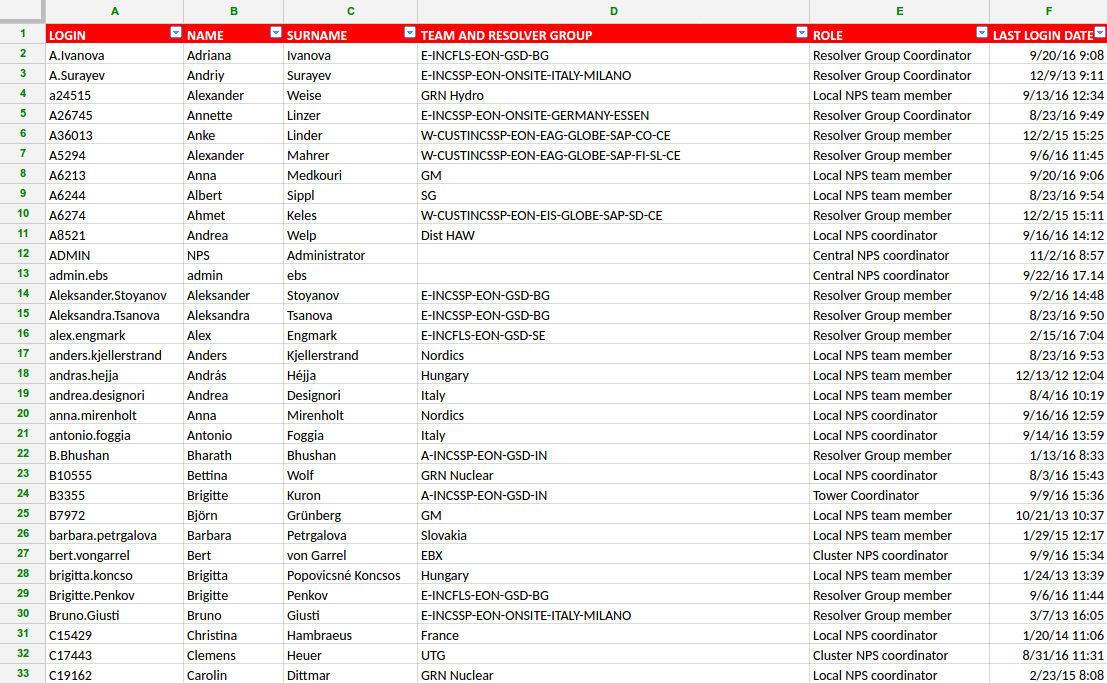
\includegraphics[scale=0.33]{UserList}
\caption{Esempio di Excel estratto contenente gli account registrati in NPS}
\label{tabella}
\end{center}
\end{figure}
\FloatBarrier


\subsection{L'importanza del database}
\label{db}
Come per tutte le applicazioni principali di Mediana S.r.l.u., anche NPS, o meglio CSIndex\footnotemark[6],
\footnotetext[6]{Nome del software così come viene venduto, come già detto nella \hyperref[prodotti]{Sezione 1.3}} è stato pensato per essere riadattabile alle esigenze di ogni nuovo cliente che lo desidera per la propria azienda. Per permettere ciò il \textit{database} è stato strutturato in modo che venga permessa la personalizzazione di ogni singolo aspetto delle varie pagine che compongono il programma, mentre la logica resta praticamente invariata, salvo quando ci sono delle nuove funzionalità non previste nella versione di base. Ciò è stato pensato anche per permettere agli sviluppatori di effettuare il più rapidamente possibile alcune modifiche che vengono richieste dal committente senza che ci sia il bisogno di effettuare ogni volta un \gls{deployment} del programma. \newpage
E in effetti così è stato anche nel mio caso, come per esempio quando mi è stato chiesto di ristrutturare il Reporting Tool\footnotemark[7]
\footnotetext[7]{Pagina dell'applicativo descritta nella \hyperref[reporting tool]{Sezione 2.3.3}}per determinati ruoli, aggiungendo o rimuovendo grafici, filtri e le diverse schede di cui esso è composto. Per fare ciò infatti, mi è bastato semplicemente aggiungere dei \textit{record} alle tabelle che permettessero di creare delle corrispondenze tra i ruoli e gli oggetti grafici descritti prima o, nel caso questi legami esistessero già, attivare dei \textit{flag} (corrispondenti ai valori 0 o 1 in una apposita colonna) per abilitarne la visualizzazione.   \\
Altro punto cardine per questo tipo di programmazione è l'implementazione di \gls{stored procedure} per manipolare ed estrarre i dati direttamente all'interno di SQL Server. Alcune di queste però non erano esenti da imperfezioni che hanno causato diversi \textit{bug}, come per esempio alcuni errori che si generavano durante la fase di estrazione oppure l'esistenza di incongruenze fra i dati estratti e quelli visualizzati all'interno dell'applicativo. In ogni caso comunque errori dovuti quasi sempre a sviste o casi limite non gestiti, risolvibili quindi con dei semplici accorgimenti.